
{\actuality} 

Определение антибиотиков в пищевых продуктах представляет собой критически важную задачу для обеспечения безопасности пищевой продукции и защиты здоровья населения. Неконтролируемое использование антибиотиков в ветеринарии приводит к их накоплению в продуктах животноводства, что создает потенциальную угрозу для здоровья человека, так как ведет к развитию антибиотикорезистентности микроорганизмов и возникновению аллергических реакций. Присутствие антибиотиков в молоке-сырье нарушает работу заквасочной культуры и может привести к браку в производстве кисломолочной продукции, что создаёт экономические риски для пищевой промышленности и обуславливает необходимость эффективного контроля качества на этапах приёмки сырья. В России установлены значения максимально допустимого уровня (МДУ) остаточного содержания  антибиотиков в продукатах питания. %ссылка

Проблема выявления остаточных количеств антибиотиков активно разрабатывается как в научной среде, так и на прикладном уровне. Существующие методы определения антибиотиков разделяют на скрининговые и подтверждающие. К подтверждающим относят высокоточные методы физико-химические методы анализа, такие как ВЭЖХ и масс-спектрометрии. Однако, стоимость оборудования и потребность в привлечении высококвалифицированного персонала ограничивает их повсеместное применение. К скрининговым методам относятся микробиологические тесты, иммуноферментный анализ (ИФА) и иммунохроматографический анализ (ИХА). Микробиологические тесты универсальны, но отличаются низкой чувствительностью и длительным временем анализа. ИФА обеспечивает высокую чувствительность и воспроизводимость, однако требует многостадийного протокола и не позволяет одновременно выявлять антибиотики разных групп. Для эффективного тестирования во внелабораторных условиях необходимо применение простых и доступных методов и быстрых методов, таких как ИХА. 

\begin{figure}[ht]
    \centerfloat{
        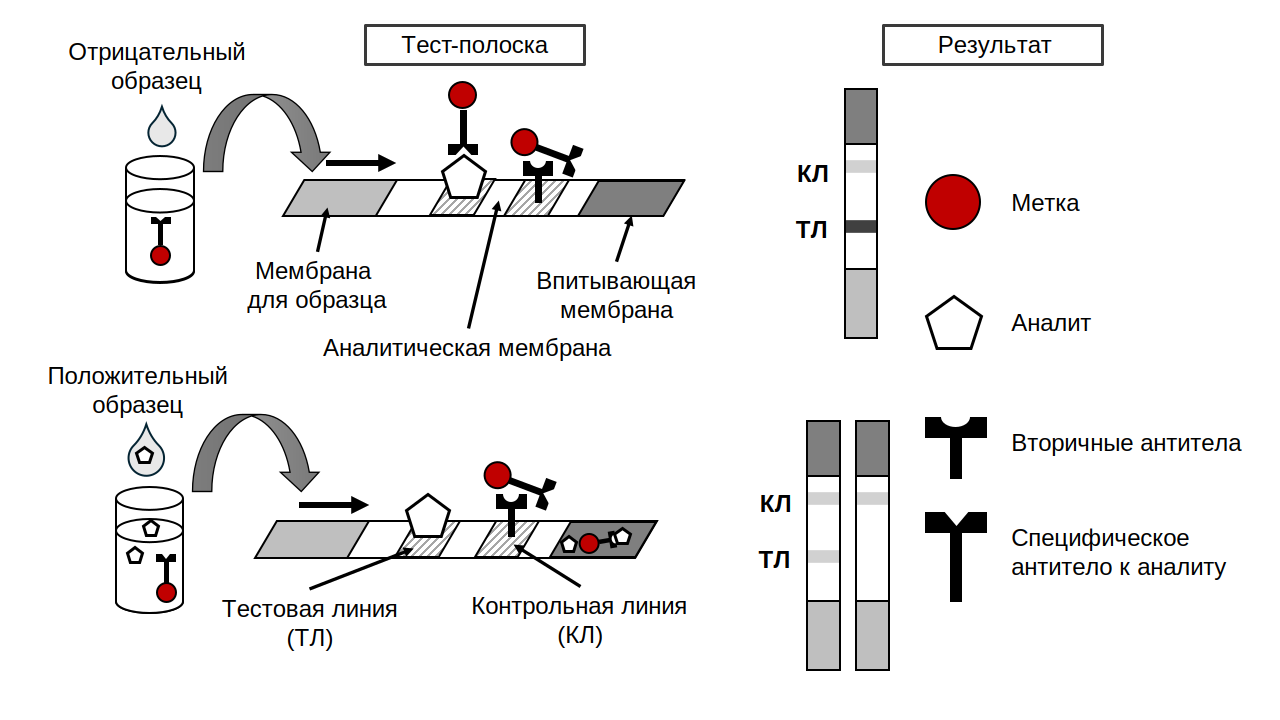
\includegraphics[scale=0.27]{с_ica_principle}
    }
    \caption{Принцип конкурентного иммунохроматографического анализа.}\label{fig:с_ica_principle}
\end{figure}

Для обнаружения малых молекул наиболее распространенным является конкурентный ИХА. Конкурентным же он назван, поскольку аналит из образца конкурирует за связывание с антителами с аналитом, закрепленном на мембране. Образец смешивается с меченными антителами, после чего переносится на тест-полоску и под действием капилярных сил протекает по аналитической мембране. При отсутствии аналита в образце антитела свяжется с аналитом, закрепленном на мембране, что приведет к аккумулированию в области метки и появлении сигнала. При наличии аналита в образце, сайт связывания антител будет уже занят и антитела уже не смогут связаться с аналитом, закрепленном на мембране. В результате этого сигнал будет отсутствовать или его интенсивность снизится (рис. \cref{fig:с_ica_principle}).  Одним из ограничений ИХА является его относительно низкая чувствительность, которая во много обусловлена несовершенством методик иммобилизации иммунореагентов и конъюгации биорецепторов с окрашивающими метками. Поэтому, разработка подходов направленных на решение вышеупомянутых проблем без утраты простоты и доступности анализа остаётся актуальной задачей биоорганической химии.

Для обнаружения антибиотиков в молоке на рынке РФ преобладают импортные тест-системы, такие как 4Sensor BSCT (Unisensor, Бельгия) и 4in1 BSCT (Bioeasy, Китай). Отечественные решения, позволяющие одновременно определять несколько групп антибиотиков в одной тест-системе, отсутствуют. Решением совета Евразийской экономической комиссии №70 от 23.06.2023 были внесены изменения в перечень контролируемых антибиотиков в продуктах питания. Перечень расширился с 4 (пенициллины, тетрациклины, хлорамфеникол, стрептомицин) до 75 наименований. В этой связи создание отечественного мультиплексного экспресс-теста для выявления антибиотиков представляется необходимым для укрепления продовольственной безопасности страны.

\progress
% Этот раздел должен быть отдельным структурным элементом по
% ГОСТ, но он, как правило, включается в описание актуальности
% темы. Нужен он отдельным структурынм элемементом или нет ---
% смотрите другие диссертации вашего совета, скорее всего не нужен.

%Такие тест-системы востребованы на фермах и перерабатывающих предприятиях для контроля качества сырья и готовой продукции. Анализ должен обеспечивать высокую чувствительность, быстрое получение результатов, простоту интерпретации при сохранении лёгкости в использовании. Несколько обобщающих работ были посвящены общим принципам разработки и ключевым задачам иммунохроматографических анализов \cite{parolo2020tutorial,hsieh2017analytical}, особенно в контексте повышения аналитической чувствительности \cite{dey2023new,omidfar2023lateral}, однако тонкие процессы оптимизации, стабильности анализа и масштабируемости технологии, к сожалению, часто остаются без должного внимания.

Научная литература отражает значительный интерес к мультиплексному ИХА-анализу~--- возможности определять несколько аналитов на одной тест-полоске \cite{di2021ten}. Например, были разработаны тест-полоски для одновременного определения свинца, водорослевого токсина, антибиотика, гормона и пестицида в питьевой воде \cite{xing2015ultrasensitive}. Для повышения чувствительности анализа могут быть применены флуоресцентные метки. Adunphatcharaphon и соавт. разработали мультиплексный флуоресцентный иммунохроматографический анализ для одновременного определения пяти микотоксинов в рисе, используя тестовые-зоны в виде точек на мембране вместо традиционных линий \cite{adunphatcharaphon2024multiplex}. Точки занимают значительно меньше места, чем тестовые-линии, что потенциально позволяет увеличить количество определяемых аналитов на одной полоске. Однако увеличение числа тестовых-зон и применение флуоресцентных меток затрудняет визуальную интерпретацию результатов, а поэтому требует использования считывающего устройства для исключения человеческого фактора при анализе.

Другим перспективным направлением повышения чувствительности ИХА является ориентированная иммобилизация антител.Использование вторичных антител (специфичных к антителам другого вида) в качестве линкеров  для иммобилизации антител к аналиту показало высокую эффективность и позволяет достигать высокой чувствительности \cite{barshevskaya2023modular,Barshevskaya2025,Sotnikov2022double}.

Несмотря на наличие ряда работ, посвящённых мультианализу, в доступной литературе не описано одновременное определение на одной тест-полоске именно тетрациклинов, стрептомицина, хлорамфеникола и пенициллина. Кроме того, большинство публикаций не раскрывают технологические аспекты подготовки стабильных и лиофилизированных иммунореагентов, что затрудняет воспроизведение описанных методик. Также не описаны нюансы масштабирования технологий приготовления коллоидного золота и конъюгатов на его основе. Настоящее исследование направлено на восполнение этих пробелов.


{\aim} данной работы является \ldots

Для~достижения поставленной цели необходимо было решить следующие {\tasks}:
\begin{enumerate}[beginpenalty=10000] % https://tex.stackexchange.com/a/476052/104425
  \item Исследовать, разработать, вычислить и~т.\:д. и~т.\:п.
  \item Исследовать, разработать, вычислить и~т.\:д. и~т.\:п.
  \item Исследовать, разработать, вычислить и~т.\:д. и~т.\:п.
  \item Исследовать, разработать, вычислить и~т.\:д. и~т.\:п.
\end{enumerate}


{\novelty}
\begin{enumerate}[beginpenalty=10000] % https://tex.stackexchange.com/a/476052/104425
  \item Впервые \ldots
  \item Впервые \ldots
  \item Было выполнено оригинальное исследование \ldots
\end{enumerate}

{\influence} \ldots

{\methods} \ldots

{\defpositions}
\begin{enumerate}[beginpenalty=10000] % https://tex.stackexchange.com/a/476052/104425
  \item Первое положение
  \item Второе положение
  \item Третье положение
  \item Четвертое положение
\end{enumerate}
В папке Documents можно ознакомиться с решением совета из Томского~ГУ
(в~файле \verb+Def_positions.pdf+), где обоснованно даются рекомендации
по~формулировкам защищаемых положений.

{\reliability} полученных результатов обеспечивается \ldots \ Результаты находятся в соответствии с результатами, полученными другими авторами.


{\probation}
Основные результаты работы докладывались~на:
перечисление основных конференций, симпозиумов и~т.\:п.

{\contribution} Автор принимал активное участие \ldots

\ifnumequal{\value{bibliosel}}{0}
{%%% Встроенная реализация с загрузкой файла через движок bibtex8. (При желании, внутри можно использовать обычные ссылки, наподобие `\cite{vakbib1,vakbib2}`).
    {\publications} Основные результаты по теме диссертации изложены
    в~XX~печатных изданиях,
    X из которых изданы в журналах, рекомендованных ВАК,
    X "--- в тезисах докладов.
}%
{%%% Реализация пакетом biblatex через движок biber
    \begin{refsection}[bl-author, bl-registered]
        % Это refsection=1.
        % Процитированные здесь работы:
        %  * подсчитываются, для автоматического составления фразы "Основные результаты ..."
        %  * попадают в авторскую библиографию, при usefootcite==0 и стиле `\insertbiblioauthor` или `\insertbiblioauthorgrouped`
        %  * нумеруются там в зависимости от порядка команд `\printbibliography` в этом разделе.
        %  * при использовании `\insertbiblioauthorgrouped`, порядок команд `\printbibliography` в нём должен быть тем же (см. biblio/biblatex.tex)
        %
        % Невидимый библиографический список для подсчёта количества публикаций:
        \phantom{\printbibliography[heading=nobibheading, section=1, env=countauthorvak,          keyword=biblioauthorvak]%
        \printbibliography[heading=nobibheading, section=1, env=countauthorwos,          keyword=biblioauthorwos]%
        \printbibliography[heading=nobibheading, section=1, env=countauthorscopus,       keyword=biblioauthorscopus]%
        \printbibliography[heading=nobibheading, section=1, env=countauthorconf,         keyword=biblioauthorconf]%
        \printbibliography[heading=nobibheading, section=1, env=countauthorother,        keyword=biblioauthorother]%
        \printbibliography[heading=nobibheading, section=1, env=countregistered,         keyword=biblioregistered]%
        \printbibliography[heading=nobibheading, section=1, env=countauthorpatent,       keyword=biblioauthorpatent]%
        \printbibliography[heading=nobibheading, section=1, env=countauthorprogram,      keyword=biblioauthorprogram]%
        \printbibliography[heading=nobibheading, section=1, env=countauthor,             keyword=biblioauthor]%
        \printbibliography[heading=nobibheading, section=1, env=countauthorvakscopuswos, filter=vakscopuswos]%
        \printbibliography[heading=nobibheading, section=1, env=countauthorscopuswos,    filter=scopuswos]}%
        %
        \nocite{*}%
        %
        {\publications} Основные результаты по теме диссертации изложены в~\arabic{citeauthor}~печатных изданиях,
        \arabic{citeauthorvak} из которых изданы в журналах, рекомендованных ВАК%
        \ifnum \value{citeauthorscopuswos}>0%
            , \arabic{citeauthorscopuswos} "--- в~периодических научных журналах, индексируемых Web of~Science и Scopus%
        \fi%
        \ifnum \value{citeauthorconf}>0%
            , \arabic{citeauthorconf} "--- в~тезисах докладов.
        \else%
            .
        \fi%
        \ifnum \value{citeregistered}=1%
            \ifnum \value{citeauthorpatent}=1%
                Зарегистрирован \arabic{citeauthorpatent} патент.
            \fi%
            \ifnum \value{citeauthorprogram}=1%
                Зарегистрирована \arabic{citeauthorprogram} программа для ЭВМ.
            \fi%
        \fi%
        \ifnum \value{citeregistered}>1%
            Зарегистрированы\ %
            \ifnum \value{citeauthorpatent}>0%
            \formbytotal{citeauthorpatent}{патент}{}{а}{}%
            \ifnum \value{citeauthorprogram}=0 . \else \ и~\fi%
            \fi%
            \ifnum \value{citeauthorprogram}>0%
            \formbytotal{citeauthorprogram}{программ}{а}{ы}{} для ЭВМ.
            \fi%
        \fi%
        % К публикациям, в которых излагаются основные научные результаты диссертации на соискание учёной
        % степени, в рецензируемых изданиях приравниваются патенты на изобретения, патенты (свидетельства) на
        % полезную модель, патенты на промышленный образец, патенты на селекционные достижения, свидетельства
        % на программу для электронных вычислительных машин, базу данных, топологию интегральных микросхем,
        % зарегистрированные в установленном порядке.(в ред. Постановления Правительства РФ от 21.04.2016 N 335)
    \end{refsection}%
    \begin{refsection}[bl-author, bl-registered]
        % Это refsection=2.
        % Процитированные здесь работы:
        %  * попадают в авторскую библиографию, при usefootcite==0 и стиле `\insertbiblioauthorimportant`.
        %  * ни на что не влияют в противном случае
        \nocite{vakbib2}%vak
        \nocite{patbib1}%patent
        \nocite{progbib1}%program
        \nocite{bib1}%other
        \nocite{confbib1}%conf
    \end{refsection}%
        %
        % Всё, что вне этих двух refsection, это refsection=0,
        %  * для диссертации - это нормальные ссылки, попадающие в обычную библиографию
        %  * для автореферата:
        %     * при usefootcite==0, ссылка корректно сработает только для источника из `external.bib`. Для своих работ --- напечатает "[0]" (и даже Warning не вылезет).
        %     * при usefootcite==1, ссылка сработает нормально. В авторской библиографии будут только процитированные в refsection=0 работы.
}

При использовании пакета \verb!biblatex! будут подсчитаны все работы, добавленные
в файл \verb!biblio/author.bib!. Для правильного подсчёта работ в~различных
системах цитирования требуется использовать поля:
\begin{itemize}
        \item \texttt{authorvak} если публикация индексирована ВАК,
        \item \texttt{authorscopus} если публикация индексирована Scopus,
        \item \texttt{authorwos} если публикация индексирована Web of Science,
        \item \texttt{authorconf} для докладов конференций,
        \item \texttt{authorpatent} для патентов,
        \item \texttt{authorprogram} для зарегистрированных программ для ЭВМ,
        \item \texttt{authorother} для других публикаций.
\end{itemize}
Для подсчёта используются счётчики:
\begin{itemize}
        \item \texttt{citeauthorvak} для работ, индексируемых ВАК,
        \item \texttt{citeauthorscopus} для работ, индексируемых Scopus,
        \item \texttt{citeauthorwos} для работ, индексируемых Web of Science,
        \item \texttt{citeauthorvakscopuswos} для работ, индексируемых одной из трёх баз,
        \item \texttt{citeauthorscopuswos} для работ, индексируемых Scopus или Web of~Science,
        \item \texttt{citeauthorconf} для докладов на конференциях,
        \item \texttt{citeauthorother} для остальных работ,
        \item \texttt{citeauthorpatent} для патентов,
        \item \texttt{citeauthorprogram} для зарегистрированных программ для ЭВМ,
        \item \texttt{citeauthor} для суммарного количества работ.
\end{itemize}
% Счётчик \texttt{citeexternal} используется для подсчёта процитированных публикаций;
% \texttt{citeregistered} "--- для подсчёта суммарного количества патентов и программ для ЭВМ.

Для добавления в список публикаций автора работ, которые не были процитированы в
автореферате, требуется их~перечислить с использованием команды \verb!\nocite! в
\verb!Synopsis/content.tex!.
